\documentclass[graphics]{beamer}

\usepackage{graphicx}
\usepackage{verbatim}
\usepackage{wrapfig}
\useoutertheme{shadow}
%\usecolortheme{orchid}
\usecolortheme{seahorse}


% math commands
\newcommand{\be}{\begin{eqnarray}}
\newcommand{\ee}{\end{eqnarray}}
\newcommand{\beq}{\begin{equation}}
\newcommand{\eeq}{\end{equation}}
\def\simless{\mathbin{\lower 3pt\hbox
      {$\rlap{\raise 5pt\hbox{$\char'074$}}\mathchar"7218$}}}
\def\simgreat{\mathbin{\lower 3pt\hbox
      {$\rlap{\raise 5pt\hbox{$\char'076$}}\mathchar"7218$}}} %> or of order

% variables

\def\toonscale{0.45}
\def\mboxy#1{\mbox{\small #1}}


\begin{comment}
\AtBeginSection[]{
  \frame{
    \frametitle{Outline}
    \tableofcontents[currentsection]
  }
}
\end{comment}

\title{Observing a bounce
}
\subtitle{}
\author[U. Pen]{\textcolor{red}{
D. Kodwani, D. Meerburg, N. Turok and more
}
\\[8mm] 
}
\date{June 26, 2017}


\begin{document}

\frame{
\begin{picture}(320,250)
\put(-5,-53){
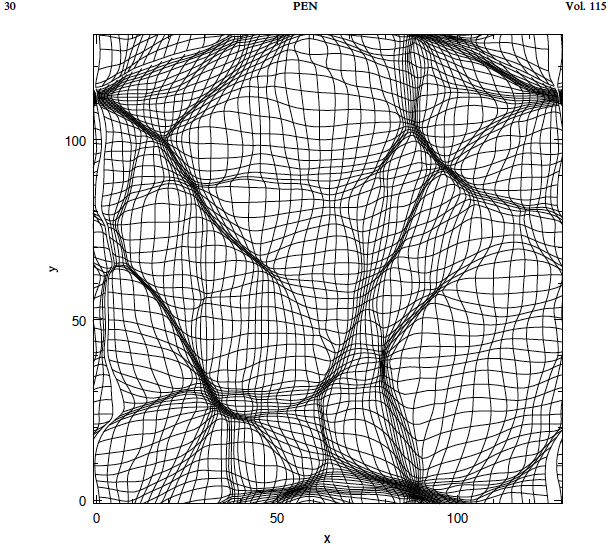
\includegraphics[width=4.5in]{Figures/mmh.png}}
\end{picture}
\vspace{-3in}
\titlepage
}

%\section*{Introduction}

\begin{comment}
  \subsection{Outline}

  \frame{
    \frametitle{Outline}
    \tableofcontents
  }
\end{comment}


\frame{
    \frametitle{Cosmological Perturbations}
    \begin{itemize}
        \item traditionally thought of as an initial value problem
        \item challenges at specifying IVP at a singularity
        \item blinded by inflationary calculations
     \end{itemize}
  }
\frame{
    \frametitle{Example: Milne Universe decaying mode}
   \begin{itemize}
   \item Milne: $\Omega=0$ hyperbolic reslicing of minkowski
\item $ds^2=-d\tau^2+\tau^2(d\chi^2/(1+\chi^2)+\chi^2 d\Omega)
        \item Gauge transform from Minkowski
        \item $r=\tau\chi$, $t=\tau \sqrt{1+\chi^2}$
     \end{itemize}

  }

\frame{
    \frametitle{3-D: E-mode}
\center{\includegraphics[width=4.3in]{Figures/delta_reco_raw.pdf}  }
  }

  \frame{
    \frametitle{Decaying modes}
\begin{itemize}
\item test fluid in Milne (empty) space:
\item has constant and decaying mode
\item if viewed backward in time, decaying mode becomes growing mode!
\item but by construction, no gravity at play.
\end{itemize}
}

\frame{
\frametitle{Tensor Modes}
\begin{itemize}
\item regular and irregular (decaying) mode
\item decaying mode $h_T \propto \cos(k\eta)/\eta$
\item viewed going into a bounce, appears as a superhorizon anistropy
\item c.f. Bianchi IX, Mixmaster
\item used as BBN constraint (Rothman\&Matzner 1984 etc)
\item if two axes expand anisotropically between neutrino freezout
  ($\sim 1$ MeV)
  and BBN ($\sim 0.1$ MeV), results in anistropic $\nu$ DF, and higher
  He abundance (up to 0.9).
\item gives stronger constraint than CMB (Saadeh et al 2016)
\end[itemize}
}

  \frame{
    \frametitle{Distinguishing gravity from fluids}
}

\frame{
\vspace{-0.5in}
    \frametitle{Conclusions}
    \begin{itemize}
      \item Non-linear backward mapping: bijiective potential isobaric coordinates
      \item most precise non-parametric reconstruction mechanism to
          date: 1-2 orders of magnitude more linear information
          \item computationally straightforward, mass coordinate
            similar to Lagrangian
        \item well suited for low shot noise low z BAO surveys,
          i.e. intensity mapping
     \end{itemize}
  }


\end{document}
